\documentclass[11pt]{article}

\usepackage{xfrac}

\input{setup}
\import{pfpl-defns/}{params}

\import{pfpl-defns/}{generic}
\import{pfpl-defns/}{icoi}
\import{pfpl-defns/}{jdg}
\import{pfpl-defns/}{lang}
\import{pfpl-defns/}{pcf}
\import{pfpl-defns/}{syn}
\import{pfpl-defns/}{t}
\import{pfpl-defns/}{ts}

\newcommand{\LangPSF}{\Lang{PSF}}

\newcommand{\intro}{\textsc{-I}}
\newcommand{\elim}{\textsc{-E}}

\newcommand{\Iso}{\simeq}
\newcommand{\N}{\mathbb{N}}

\newcommand{\ltrue}{\top}
\newcommand{\lfalse}{\bot}
\newcommand{\limplies}{\supset}
\newcommand{\liff}{\supset\subset}

\input{issolution}

\title{Assignment 2: \\
       Induction, Coinduction, and Recursion}

\begin{document}

\maketitle

In this assignment, we'll explore \emph{generic programming} with inductive and coinductive types, embedded in Standard~ML.
In functional programming lingo, this technique is often called ``recursion schemes''.%
\footnote{
  To learn more, see:
  \begin{itemize}
    \item \href{https://www.cs.cmu.edu/~tom7/papers/wang-murphy-recursion.pdf}{Functional Pearl: Programming with Recursion Schemes (Wang and Murphy)}
    \item \href{https://maartenfokkinga.github.io/utwente/mmf91m.pdf}{Functional Programming with Bananas, Lenses, Envelopes and Barbed Wire (Meijer, Fokkinga, and Paterson)}
    \item \href{https://blog.sumtypeofway.com/posts/introduction-to-recursion-schemes.html}{An Introduction to Recursion Schemes (Thomson)}
  \end{itemize}
  }
We will then consider how to formally prove code using inductive and coinductive types by induction and coinduction, respectively.
Finally, we will briefly consider partiality in \LangPCF{}.


\section{Type Operators}

First, we will briefly introduce \emph{type operators}, which wil allow us to share common utilities across implementations of inductive and coinductive types.

\begin{figure}[h]
  \codefile[linerange={1-2,4-5}]{recursion-schemes/generic/positive-type-operator.sig}
  \caption{Signature for type operators}
  \label{fig:type-operator}
\end{figure}

In \cref{fig:type-operator}, we reproduce the typeclass \code{TYPE_OPERATOR}.%
\footnote{In \PFPL, this is written $\AbsABT{t}{\tau}$, where $\tau$ is the \code{view} type.}
A type operator is simply a parameterized type \code{'t view}, which we will use to define the ``shape'' of the induction (or coinduction).
On this assignment, we will use \code{signature POSITIVE_TYPE_OPERATOR}, which extends \code{TYPE_OPERATOR} slightly.%
\footnote{The positivity requirement guarantees that \code{view} is ``functorial'', i.e., has a structure-preserving \code{map} function. For more details, see \PFPL[14].}

\begin{figure}[h]
  \codefile[linerange={1-3,9-9}]{recursion-schemes/experiments/type-ops.sml}
  \caption{Type operator for natural numbers}
  \label{fig:nat-op}
\end{figure}

Let's look at a simple example, the type operator for natural numbers, in \cref{fig:nat-op}.
We define \code{'t view} to have two cases, \code{Zero} and \code{Succ}.
However, notice that \code{'t view} is \emph{not} recursive!
In place of where we would like to ``recur'' (in the \lstinline{Succ} case), we include the type variable \lstinline{'t}.
In \cref{sec:inductive}, we will see how to use \code{NatOp} to define the natural numbers; then, \code{Zero} and \code{Succ} will behave somewhat like constructors.


\section{Inductive Types}\label{sec:inductive}

Now, we will consider inductive types.
In our setup, we will define inductive types ``generically'' (in a common library) based around type operators.
This will allow us to reuse infrastructure across all inductive types, including natural numbers, lists, and trees.

\begin{figure}[h]
  \codefile[linerange={1-2,4-5,7-8,14-15,21-22}]{recursion-schemes/generic/inductive.sig}
  \caption{Signature for inductive types}
  \label{fig:inductive}
\end{figure}

In \cref{fig:inductive}, we show the signature for generalized inductive types.
First, we have some type operator parameter \code{structure T}.
We also have an abstract type \code{t} that will be the least fixed point of \code{T}; in other words, the ``inductively iterated'' version of \code{T}.%
\footnote{In \PFPL[15], this is written $\indtycst{t}{\tau}$.}
Finally, we have the expected operations: the generalized constructor \code{FOLD} and the recursor \code{REC}.
We use \code{'rho}/$\rho$ for the \colorbox{yellow}{\textbf{r}}esult type of the recursor.

{\color{red}\textbf{IMPORTANT:}}
To get points for these tasks, you must \emph{not} use any explicit recursion in Standard~ML (e.g., \code{fun}) or any built-in infinite datatypes (e.g., \code{int}).
You should only use the provided inductive types and their recursors.

Throughout this section, you will work in \path{recursion-schemes/experiments/experiments.fun}.
See \path{recursion-schemes/experiments/experiments.sig} for the signature to implement.
You can find the relevant type operators in \path{recursion-schemes/experiments/type-ops.sml}.

\subsection{Natural Numbers}

Let us consider natural numbers, defined as a \code{structure Nat : INDUCTIVE where T = NatOp} (i.e., letting the \code{structure T} be \code{NatOp} from \cref{fig:nat-op}).
There is a key difference between \code{NatOp} and \code{Nat}: the former describes a ``template'', whereas the second describes the inductive type of natural numbers.
Using the two together, we may define:
\begin{align*}
  \nattycst &\isdef{} \code{Nat.t} \\
  \zerocst &\isdef{} \code{Nat.FOLD NatOp.Zero} \\
  \succcst{\code{n}} &\isdef{} \code{Nat.FOLD (NatOp.Succ n)} \\
  \natiterabt{\rho}{\code{n}}{\code{e0}}{\code{x}}{\code{e1}} &\isdef{} \code[mathescape=true]{Nat.REC (fn NatOp.Zero => e0 | NatOp.Succ x => e1)$\ $ n}
\end{align*}
Observe that the constructors $\zerocst$ and $\succcst{\code{n}}$ are combined into one unified recursive constructor, \code{FOLD}, separating the inductive code on \code{Nat.t} from the sum type \code{'t NatOp.view}.
Similarly, the base case \code{e0} and the inductive case $\AbsABT{\code{x}}{\code{e1}}$ are combined into the parameter of \code{REC}.
Note that \code{x} has type $\rho$, not $\nattycst$: the inductive result is put in all \code{'t} positions.
This will generalize naturally to data structures with multiple recursive sub-components, such as trees, where each inductively-computed result will be in the corresponding \code{view} position.

\begin{remark}
  One may be tempted to say, for example, \code{Nat.T.Zero} instead of \code{NatOp.Zero}; however, although it is known that \code{Nat.T = NatOp}, one quirk of Standard~ML is that the constructors \code{Zero} and \code{Succ} are not available under \code{Nat.T} since \code{Nat.T : INDUCTIVE}.
\end{remark}

\begin{figure}[h]
  \begin{codeblock}
  type nat = Nat.t

  val ZERO : nat        = Nat.FOLD N.Zero
  val SUCC : nat -> nat = Nat.FOLD o N.Succ

  val double : nat -> nat =
    Nat.REC
      (fn N.Zero   => ZERO
        | N.Succ n => SUCC (SUCC n))

  val add : nat * nat -> nat =
    fn (m, n) =>
      Nat.REC
        (fn N.Zero   => n
          | N.Succ r => SUCC r)
        m
  \end{codeblock}
  \caption{Simple functions on natural numbers, where \code{structure N = NatOp}}
  \label{fig:nat-functions}
\end{figure}
In \cref{fig:nat-functions}, we define some basic functions on natural numbers using convenience functions \code{ZERO} and \code{SUCC}.
The \code{double} code is straightforward; we assume that our inductive result has already been computed in the \code{Succ} case.
In \code{add}, we elect (here, without loss of generality) to go by induction on \code{m}, using \code{n} in the base case.

\begin{task}{15}
  In \path{recursion-schemes/experiments/experiments.fun}, complete the definition of \code{NatUtil}.
  In particular:
  \begin{itemize}
    \item \code{exp2 n} should compute the \code{n}$^\text{th}$ power of $2$.
    \item \code{halve n} should compute the floor of $\frac{\code{n}}{2}$.
    \item \code{fib n} should compute the \code{n}$^\text{th}$ Fibonacci number $F_n$, where $F_0 = 0$, $F_1 = 1$, and $F_{n+2} = F_n + F_{n+1}$.
  \end{itemize}
\end{task}
\begin{hint}
  You should be able to implement \code{exp2} in a straightforward manner using \code{double}.
  For \code{halve} and \code{fib}, you may wish to consider strengthening your inductive hypothesis, computing more than you need.
  You are welcome to use finite products and sums in Standard~ML, such as booleans and pairs.
\end{hint}

\paragraph{Testing}
If you open the SML/NJ REPL, you can test your code via \code{structure Experiments}, an instantiation of your \code{functor Experiments}.
It is instantiated such that \code{Nat.t} is in fact \code{int}, allowing you to test easily.
\begin{codeblock}
  smlnj -m sources.cm
  - open Experiments;
  - NatUtil.exp2 0;
  val it = 1 : nat
  - NatUtil.exp2 10;
  val it = 1024 : nat
  - NatUtil.halve 312;
  val it = 156 : nat
  - NatUtil.halve 313;
  val it = 156 : nat
  - NatUtil.fib 14;
  val it = 377 : nat
\end{codeblock}

\subsection{Lists}\label{sec:lists}

Now, let's consider another inductive types: lists of natural numbers.

\begin{figure}[h]
  \begin{codeblock}
  structure ListOp =
    struct
      type element = Nat.t
      datatype 't view = Nil | Cons of element * t
    end
  \end{codeblock}
  \caption{Type operator for lists}
  \label{fig:list-op}
\end{figure}

Just as with natural numbers, we first define the ``type operator'', concisely reproduced in \cref{fig:list-op}.
Then, we include a \code{structure List : INDUCTIVE where T = ListOp}.

\begin{figure}[h]
  \begin{codeblock}
  type list = List.t

  val length : list -> nat =
    List.REC
      (fn L.Nil => ZERO
        | L.Cons (_, n) => SUCC n)

  val map : (element -> element) -> list -> list =
    fn f =>
      List.REC
        (fn L.Nil          => List.FOLD L.Nil
          | L.Cons (x, xs) => List.FOLD (L.Cons (f x, xs)))
  \end{codeblock}
  \caption{Sample functions on lists of natural numbers, where \code{structure L = ListOp}}
  \label{fig:list-functions}
\end{figure}
We show the implementation of some sample list functions in \cref{fig:list-functions}.

\begin{task}{10}
  In \path{recursion-schemes/experiments/experiments.fun}, implement:
  \begin{itemize}
    \item \code{ListUtil.sum l} to compute the sum of \code{l} (using \code{NatUtil.add}).
    \item \code{ListUtil.filter p l} to compute a list of the elements in \code{l} satisfying and not satisfying \code{p}, in the order they appear in \code{l}. It should behave like \code{List.filter} from the Standard~ML Basis Library.
  \end{itemize}
\end{task}

\begin{task}{10}
  In \path{recursion-schemes/experiments/experiments.fun}, implement the function \code{ListUtil.reverse} such that \code{reverse l} reverses the list \code{l}, a la \code{List.rev}.
  Your implementation should run in linear time in terms of the length of the list; a super-linear runtime solution will earn you partial credit.
\end{task}
\begin{hint}
  You may find it useful to recall the recursive implementation of list reverse:
\begin{lstlisting}
  fun reverseHelper nil       acc = acc
    | reverseHelper (x :: xs) acc = reverseHelper xs (x :: acc)

  fun reverse l = reverseHelper l nil
\end{lstlisting}

  You may want to refresh your memory on CPS from 15-150; consider accumulating a function.
\end{hint}

\paragraph{Testing}
Once again, you can test your code via \code{structure Experiments}.
It instantiates your \code{functor Experiments} such that \code{List.t} is in fact \code{int list}, allowing you to test easily.
\begin{codeblock}
  smlnj -m sources.cm
  - open Experiments;
  - ListUtil.sum [1, 5, 3, 1, 2];
  val it = 12 : int
  - ListUtil.filter (fn x => x <= 2) [1, 5, 3, 1, 2];
  val it = [1,1,2] : int list
\end{codeblock}

\subsubsection{Derived Forms}

Thus far, the functions we have asked you to consider have been fairly amenable to simple inductive implementation.
However, not all code is so straightforward!
For example, we often wish to pattern match on the outer layer of a list.
Additionally, we sometimes want immediate access to our predecessor, as included natively in the \LangT{} recursor.
While neither of these operations are present as primitives, we can implement them as \emph{derived forms}.

\begin{task}{10}
  In \path{recursion-schemes/experiments/experiments.fun}, implement the function \code{ListUtil.UNFOLD : list -> list ListOp.view}, which will allow us to unwrap one layer of a list and pattern match immediately on \code{ListOp.Nil} and \code{ListOp.Cons}.
  Concretely, \code{UNFOLD (List.FOLD v)} should evaluate to \code{v : list ListOp.view}.
\end{task}
\begin{hint}
  Consider going by induction (i.e., \code{REC}).
\end{hint}

\begin{task}{10}
  In \path{recursion-schemes/experiments/experiments.fun}, implement the function \code[mathescape=true]{ListUtil.REC' : (('rho * list)$\ $ ListOp.view -> 'rho)$\ $ -> list -> 'rho}, which will be similar to \code{REC} while also providing us with the list tail at each layer.

  \begin{figure}
  \begin{codeblock}
  fun stripLeading p nil = nil
    | stripLeading p (x :: xs) =
        if p x
          then stripLeading p xs
          else x :: xs

  val stripLeading : (element -> bool) -> list -> list =
    fn p =>
      ListUtil.REC'
        (fn ListOp.Nil => List.FOLD ListOp.Nil
          | ListOp.Cons (x, (res, xs)) =>
              if p x
                then res
                else List.FOLD (ListOp.Cons (x, xs)))
  \end{codeblock}
  \caption{Sample usage of \code{ListUtil.REC'}}
  \label{fig:rec'}
  \end{figure}
  The usage of \code{REC'} shown in \cref{fig:rec'} should be identical to the corresponding recursive Standard~ML code.
\end{task}
\begin{hint}
  Consider ``strengthening your IH'': in addition to computing not only the desired result, you may wish to inductively reconstruct the list itself.
\end{hint}

\subsubsection{Insertion Sort}

Let's implement insertion sort inductively.
First, recall its usual implementation in \cref{fig:insertion-sort}.
\begin{figure}
\begin{codeblock}
  fun insert (x, nil    ) = x :: nil
    | insert (x, y :: ys) =
        if x <= y
          then x :: y :: ys
          else y :: insert (x, ys)

  fun sort nil       = nil
    | sort (x :: xs) = insert (x, sort xs)
\end{codeblock}
\caption{Insertion sort, recursively}
\label{fig:insertion-sort}
\end{figure}

\begin{task}{20}
  In \path{recursion-schemes/experiments/experiments.fun}, implement the structure \code{InsertionSort}.
  In particular, you should define \code{insert} and \code{sort} to mirror the above definitions.
  The comparison function \code{<=} is provided at the top of the file.
\end{task}
\begin{hint}
  In the second case of \code{insert}, you sometimes return \code{x :: y :: ys}, where \code{ys} is unchanged.
  Which of the previously-defined derived forms might help you accomplish this?
\end{hint}

\subsubsection{Merge Sort}

While insertion sort is structurally recursive, one might wonder: how could we implement an algorithm like merge sort, which recurs on lists which are not the immediate tail?
Recall its implementation in \cref{fig:merge-sort}.
\begin{figure}
\begin{codeblock}
  fun split nil       = (nil, nil)
    | split (x :: xs) =
        let
          val (l1, l2) = split xs
        in
          (l2, x :: l1)
        end

  fun merge (nil    , l2     ) = l2
    | merge (l1     , nil    ) = l1
    | merge (x :: xs, y :: ys) =
        if x <= y
          then x :: merge (xs, y :: ys)
          else y :: merge (x :: xs, ys)

  fun sort nil = nil
    | sort (x :: nil) = x :: nil
    | sort (x :: xs) =
        let
          val (l1, l2) = split (x :: xs)
        in
          merge (sort l1, sort l2)
        end
\end{codeblock}
\caption{Merge sort, recursively}
\label{fig:merge-sort}
\end{figure}

Consider \code{sort}: in the last case, we recursively sort \code{l1} and \code{l2}.
To implement this behavior using the recursor, we use a clever trick: we go by induction not on the list itself, but on a ``clock'' indicating the desired recursion depth.

\begin{figure}
\begin{codeblock}
  val sort : list -> list =
    fn l =>
      Nat.REC
        (fn N.Zero => (fn l => l)
          | N.Succ f =>
              fn l =>
                let
                  val (l1, l2) = split l
                in
                  merge (f l1, f l2)
                end)
        (ListUtil.length l)
        l
\end{codeblock}
\caption{Merge sort, inducting on a ``clock''}
\label{fig:merge-sort-clock}
\end{figure}

This approach is shown in \cref{fig:merge-sort-clock}.
Here, we recursively compute a function of type \code{list -> list}, with a specification that at inductive layer $k$, we produce a correct sorting function for lists of length up to $2^k$.
\begin{enumerate}
  \item In the base case $k = 0$, the identity function suffices, since it sorts lists of length $0$ and $1$.
  \item In the inductive case $k = k' + 1$, we implement the usual algorithm, using an inductively-computed \code{f} capable of sorting lists of size $2^{k'}$ on the smaller lists.
\end{enumerate}
We start the recursion with $k = \code{length l}$ and apply the resulting function to \code{l}.

\begin{task}{5}
  In the above code, we start with $k = \code{length l}$; while this is a sufficiently large value of $k$ to correctly sort, it is far larger than necessary, causing the code to recur on empty and singleton lists repeatedly.
  What would be an efficient starting value for $k$ in terms of \code{l}?
  You may ignore small constants/off-by-one issues.
  Explain briefly (in 1-2 sentences).
\end{task}
\solution{sort-depth}

\begin{task}{20}
  In \path{recursion-schemes/experiments/experiments.fun}, implement \code{merge} in the structure \code{MergeSort}.
\end{task}
\begin{hint}
  You will almost certainly need to use the aforementioned technique, going by induction on a clock rather than by structural induction on one of the lists.
  Additionally, you may find one of the derived forms implemented earlier particularly useful.
\end{hint}


\section{Coinductive Types}

Let us now shift our attention to coinductive types.
\begin{figure}[h]
  \codefile[linerange={1-2,4-5,7-8,14-15,21-22}]{recursion-schemes/generic/coinductive.sig}
  \caption{Signature for coinductive types}
  \label{fig:coinductive}
\end{figure}
We will reuse the ``type operator'' infrastructure, considering a new \code{COINDUCTIVE} signature in \cref{fig:coinductive}.
As in \code{INDUCTIVE}, we have a type operator parameter \code{structure T}.
We also have an abstract type \code{t}, but this time, it will be the \emph{greatest} fixed point of \code{T}, allowing for infinite elements.%
\footnote{In \PFPL[15], this is written $\coitycst{t}{\tau}$.}
Finally, we have the expected operations: the generator \code{GEN} and the generalized destructor \code{UNFOLD}.
We use \code{'sigma}/$\sigma$ for the \colorbox{yellow}{\textbf{s}}tate type of the generator.

\begin{remark}
  Inductive and coinductive types are ``dual'' in a mathematically precise way.
  You may have already noticed the similarity between \code{INDUCTIVE} and \code{COINDUCTIVE}: they are identical, except with (some) function arrows reversed!
\end{remark}

{\color{red}\textbf{IMPORTANT:}}
To get points for these tasks, you must \emph{not} use any explicit recursion in Standard~ML (e.g., \code{fun}) or any built-in infinite datatypes (e.g., \code{int}).
You should only use the provided (co)inductive types and their recursors/generators.

\subsection{Streams}\label{sec:streams}

Using the \code{ListOp} type operator from \cref{sec:lists}, we can define potentially-infinite streams via a \code{structure Stream : COINDUCTIVE where T = ListOp}.

When working with inductive types, we used \code{FOLD} to create finite data structures layer by layer, allowing \code{REC} to ``tear down'' the entirety of the data structure.
Dually, when working with coinductive types, we will create (potentially) infinite data structures in their entirety using \code{GEN}, allowing \code{UNFOLD} to make finitely many observations about the data structure layer by layer.

In \cref{fig:list-functions}, we implemented \code{map}, which applies a function to every element of a list, by recursing over an existing list.
We implement an analogous \code{map} function on streams in \cref{fig:stream-functions}.
In particular, we use \code{Stream.GEN} with an internal state of type \code{stream}; at each layer, we mirror the structure of the state stream, applying the function \code{f} to each element.
\begin{figure}
  \begin{codeblock}
  type stream = Stream.t

  val map : (element -> element) -> stream -> stream =
    fn f =>
      Stream.GEN
        (fn s =>
          case Stream.UNFOLD s of
            L.Nil          => L.Nil
          | L.Cons (x, xs) => L.Cons (f x, xs))
  \end{codeblock}
  \caption{Simple function on streams of natural numbers, where \code{structure L = ListOp}}
  \label{fig:stream-functions}
\end{figure}

\begin{task}{10}
  In \path{recursion-schemes/experiments/experiments.fun}, implement the remaining functions in \code{structure StreamUtil}.
  \begin{itemize}
    \item
      \code{fromList l} should produce a (finite) stream which produces the elements from \code{l} in order.

    \item
      \code{zipWith f (s1, s2)} should provide a stream which produces a stream consisting of the elements of \code{s1} and \code{s2} combined pairwise with \code{f}, a la \code{ListPair.map}.
      If either stream terminates, the entire stream should terminate.
  \end{itemize}
\end{task}
\begin{hint}
  You may find \code{ListUtil.UNFOLD} helpful in \code{fromList}.
\end{hint}

\paragraph{Testing}
You can, once again, test your code via \code{structure Experiments}.
We provide a special implementation of streams which makes the front visible.
\begin{codeblock}
  smlnj -m sources.cm
  - open Experiments;
  - StreamUtil.fromList [1, 5, 3, 1, 2];
  val it = HIDE ([1,5,3,1,2],NONE) : stream
  - val squares = Stream.GEN (fn i => ListOp.Cons (i * i, i + 1)) 0;
  val squares = HIDE ([0,1,4,9,16,25,36,...],SOME fn) : Stream.t
  - StreamUtil.map (fn i => i + 1) squares;
  val it = HIDE ([1,2,5,10,17,26,37,...],SOME fn) : stream
  - StreamUtil.zipWith (op +) (squares, StreamUtil.fromList [1, 5, 3, 1, 2]);
  val it = HIDE ([1,6,7,10,18],NONE) : stream
\end{codeblock}

In \cref{sec:lists}, we considered \code{map} and \code{filter} on lists.
However, while we wrote \code{map} on streams, it is impossible to write an analogous \code{filter} function on streams using only the \code{COINDUCTIVE} interface.

\begin{task}{5}
  Briefly explain why it is impossible to write a \code{filter} function on (coinductively-defined) streams.
\end{task}
\begin{hint}
  Try writing it, and see where you get stuck!
\end{hint}
\begin{remark}
  It \emph{is} possible to write a \code{filter} function on streams using general recursion.
  (In fact, you may recall this from 15-150.)
\end{remark}
\solution{stream-filter}

\subsection{Automata}

Using our framework for coinductive types, we can elegantly describe and understand strings and automata.

An \emph{automaton} ``reads'' through a string character by character and decides whether it should \emph{reject} or \emph{accept} the string.
Every automaton works on some set of internal states, each of which is either \emph{accepting} or \emph{rejecting}.
An automaton starts in one state; when it reads a character from the string, it makes a transition to a new state according to the character it just read.
After it processed all characters in the string, it accepts the string if and only if it ends up in an accepting state.

\begin{figure}
  \centering
  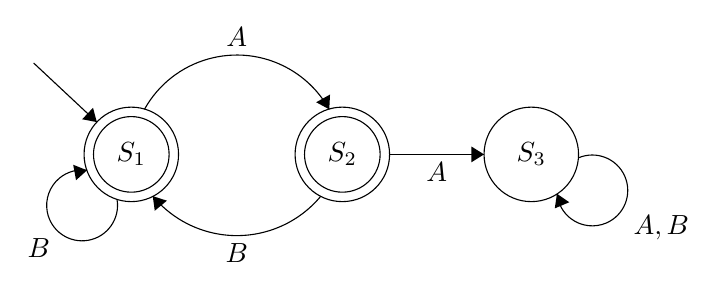
\begin{tikzpicture}[scale=0.2]
    \tikzstyle{every node}+=[inner sep=0pt]
    \draw [black] (17.1,-23) circle (3);
    \draw (17.1,-23) node {$S_1$};
    \draw [black] (17.1,-23) circle (2.4);
    \draw [black] (30.5,-23) circle (3);
    \draw (30.5,-23) node {$S_2$};
    \draw [black] (30.5,-23) circle (2.4);
    \draw [black] (42.5,-23) circle (3);
    \draw (42.5,-23) node {$S_3$};
    \draw [black] (17.932,-20.144) arc (150.94658:29.05342:6.712);
    \fill [black] (29.67,-20.14) -- (29.72,-19.2) -- (28.84,-19.69);
    \draw (23.8,-16.19) node [above] {$\kw{A}$};
    \draw [black] (16.191,-25.847) arc (10.02915:-277.97085:2.25);
    \draw (11.23,-28.34) node [below] {$\kw{B}$};
    \fill [black] (14.29,-24.01) -- (13.41,-23.66) -- (13.59,-24.64);
    \draw [black] (10.9,-17.2) -- (14.91,-20.95);
    \fill [black] (14.91,-20.95) -- (14.67,-20.04) -- (13.98,-20.77);
    \draw [black] (29.139,-25.647) arc (-39.61326:-140.38674:6.93);
    \fill [black] (18.46,-25.65) -- (18.59,-26.58) -- (19.36,-25.94);
    \draw (23.8,-28.66) node [below] {$\kw{B}$};
    \draw [black] (33.5,-23) -- (39.5,-23);
    \fill [black] (39.5,-23) -- (38.7,-22.5) -- (38.7,-23.5);
    \draw (36.5,-23.5) node [below] {$\kw{A}$};
    \draw [black] (45.48,-23.225) arc (113.42077:-174.57923:2.25);
    \draw (48.96,-27.69) node [right] {$\kw{A,B}$};
    \fill [black] (44.13,-25.5) -- (43.99,-26.43) -- (44.91,-26.04);
  \end{tikzpicture}
  \caption{State diagram for machine $M_{\lnot\kw{AA}}$. For simplicity, we use $\kw{B}$ to represent non-$\kw{A}$ characters.}
  \label{dfa:m-no-aa}
\end{figure}

As an example, the automaton $M_{\lnot\kw{AA}}$ in \cref{dfa:m-no-aa} accepts a string iff it does not contain consecutive $\kw{A}$s.
Here $S_1$ is the starting state and $S_1$ and $S_2$ are accepting states.
It accepts strings \code{""}, \code{"B"}, \code{"ABBA"}, \code{"ABA"}, but not strings \code{"AA"}, \code{"BAA"}, \code{"BBABAAB"}.
$M_{\lnot\kw{AA}}$ has three states.
It starts in $S_1$. Its accepting states include $S_1$ and $S_2$.

Now, we shall choose representations of strings and automata.
\begin{enumerate}
  \item
    Strings will be an inductive type, defineed as lists of characters.
    Specifically, \code{StringOp} will be equivalent to \code{ListOp} from \cref{fig:list-op} but with \code{type element = char}.
  \item
    Automata will be a coinductive type based around type operator \code{AutomatonOp} in \cref{fig:automaton-op}.
    In other words, an automaton will be a \code{bool}, saying whether or not the current state is ``accepting'' or not, and a transition function from a \code{char} to another automaton.
    Notice that an automaton behaves much like a stream, but with one tail available for each \code{char}.
\end{enumerate}

\begin{figure}[h]
  \begin{codeblock}
  structure AutomatonOp =
    struct
      type 't view = bool * (char -> 't)
    end
  \end{codeblock}
  \caption{Type operator for automata}
  \label{fig:automaton-op}
\end{figure}

First, we will define a function \code{run : automaton -> string -> bool}, allowing us to run an automaton on a string.

\begin{task}{15}
  In \path{recursion-schemes/experiments/experiments.fun}, implement the \code{run} function in \code{structure AutomatonUtil} according to the informal specification above.
  Your automaton should read from the ``end'' of the string first, which will visually be at the beginning.
\end{task}

\paragraph{Testing}
You can test your code via \code{structure Experiments}, where we implement \code{String} via built-in strings for convenience.
In the starter code, we define $M_{\lnot\kw{AA}}$ as \code{notConsecutiveA}.
Additionally, we provide an example \code{abc}, the automaton that accepts only the string \code{"ABC"}.
\begin{codeblock}
  smlnj -m sources.cm
  - open Experiments;
  - open AutomatonUtil;
  - run notConsecutiveA "ABBA";
  val it = true : bool
  - run notConsecutiveA "BBABAAB";
  val it = false : bool
  - run abc "ABC";
  val it = true : bool
  - run abc "ABCD";
  val it = false : bool
\end{codeblock}

Now, to implement some more automata!

\begin{task}{15}
  In \path{recursion-schemes/experiments/experiments.fun}, implement:
  \begin{itemize}
    \item \code{endsWithA : automaton} such that \code{run endsWithA} accepts all strings that end with \code{"A"}.
    \item \code{abStar : automaton} such that \code{run abStar} accepts the strings in language:
    $$\code{"AB"}^\star = \{ \code{""}, \code{"AB"}, \code{"ABAB"}, \code{"ABABAB"}, \dots \}$$
    \item \code{either : automaton * automaton -> automaton} such that \code{run (either (a1, a2))} accepts the strings that at least one of \code{a1} and \code{a2} accept.
  \end{itemize}
  You are welcome to define a custom (finite) datatype if you wish, as in examples \code{notConsecutiveA} and \code{abc}.
\end{task}

\begin{codeblock}
  smlnj -m sources.cm
  - open Experiments;
  - open AutomatonUtil;
  - run endsWithA "BA";
  val it = true : bool
  - run endsWithA "AB";
  val it = false : bool
  - run endsWithA "";
  val it = false : bool
  - run abStar "";
  val it = true : bool
  - run abStar "AB";
  val it = true : bool
  - run abStar "ABA";
  val it = false : bool
  - run (either (notConsecutiveA, endsWithA)) "AB";
  val it = true : bool
  - run (either (notConsecutiveA, endsWithA)) "BBAA";
  val it = true : bool
  - run (either (notConsecutiveA, endsWithA)) "BBAAB";
  val it = false : bool
\end{codeblock}


\section{Proof by Induction and Coinduction}

Inductive and coinductive types are, unsurprisingly, conducive to proof by induction and coinduction, respectively.
In this part of the assignment, we will prove properties about operations on inductive and coinductive data.

\subsection{Induction}

We define list length and append functions as follows, using the infrastructure described in \cref{sec:lists}:

\begin{codeblock}
  structure N = NatOp
  structure L = ListOp

  type nat = Nat.t
  type list = List.t

  val ZERO = Nat.FOLD N.Zero
  val SUCC = Nat.FOLD o N.Succ

  val length : list -> nat =
    List.REC
      (fn L.Nil => ZERO
        | L.Cons (_, n) => SUCC n)

  val append : list * list -> list =
    fn (l1, l2) =>
      List.REC
        (fn L.Nil => l2
          | L.Cons (x, l) => List.FOLD (L.Cons (x, l)))
      l1

  val add : nat * nat -> nat =
    fn (m, n) =>
      Nat.REC
        (fn N.Zero   => n
          | N.Succ r => SUCC r)
        m
\end{codeblock}

The definition of lists as an inductive type tells us that:
\begin{align*}
  \code{List.REC f (List.FOLD L.Nil)} &= \code{f L.Nil} \\
  \code{List.REC f (List.FOLD (L.Cons (x, xs)))} &= \code{f (L.Cons (x, List.REC f xs))}
\end{align*}

Since \code{list} is an inductive type, we can rigorously define what it means to go by induction on a value of type \code{list}.
The induction principle works just like \code{REC}, ``tearing down'' a list to get a desired result in each case.

\fbox{\begin{minipage}{\textwidth}
  \begin{defn}[Induction Principle for $\texttt{list}$]
    Consider some property on lists, $P(-)$.

    If it is the case that:
    \begin{quote}
      If we assume that for all values \code{v : list L.view}, either:
      \begin{enumerate}
        \item $\code{v} \isdef \code{L.Nil}$
        \item $\code{v} \isdef \code{L.Cons (x, xs)}$, where $P(\code{xs})$
      \end{enumerate}
      then, $P(\code{List.FOLD v})$ holds.
    \end{quote}
    then for all \code{l : list}, $P(\code{l})$.
  \end{defn}
\end{minipage}}

For the rest of the problem, we will abbreviate \code{List.FOLD} as \code{FOLD} and \code{List.REC} as \code{REC}.

Let's use the induction principle to prove a simple theorem.

\begin{theorem}
  For all values \code{l : list}, $\code{append (l, FOLD L.Nil)} = \code{l}$.
\end{theorem}
\begin{proof}
  We use the induction principle for \code{list}, where
  $$P(\code{l}) \isdef{} \code{append (l, FOLD L.Nil)} = \code{l}$$

  Let \code{v : list L.view} be arbitrary, and assume that either
  \begin{enumerate}
    \item $\code{v} \isdef \code{L.Nil}$
    \item $\code{v} \isdef \code{L.Cons (x, xs)}$, where $\code{append (xs, FOLD L.Nil)} = \code{xs}$
  \end{enumerate}
  It remains to show that $\code{append (FOLD v, FOLD L.Nil)} = \code{FOLD v}$.

  We go by cases on the assumption:
  \begin{enumerate}
    \item
      Suppose $\code{v} \isdef \code{L.Nil}$.
      Then:
      \begin{align*}
        &\ \code{append (FOLD v, FOLD L.Nil)} \\
        &= \code{append (FOLD L.Nil, FOLD L.Nil)} \\
        &= \code[mathescape=true]{REC (fn L.Nil => l2 | L.Cons (x, l)$\ $ => ...)$\ $ (FOLD L.Nil)} \\
        &= \code{FOLD L.Nil}  \tag*{(\code{REC} law)}
      \end{align*}
      as desired.

    \item
      Suppose $\code{v} \isdef \code{L.Cons (x, xs)}$, where $\code{append (xs, FOLD L.Nil)} = \code{xs}$.
      Then:
      \begin{align*}
        &\ \code{append (FOLD v, FOLD L.Nil)} \\
        &= \code{append (FOLD (L.Cons (x, xs)), FOLD L.Nil)} \\
        &= \code[mathescape=true]{REC (fn L.Nil => l2 | L.Cons (x, l)$\ $ => ...)$\ $ (FOLD (L.Cons (x, xs)))} \\
        &= \code{FOLD (L.Cons (x, append (xs, FOLD L.Nil)))}  \tag*{(\code{REC} law)} \\
        &= \code{FOLD (L.Cons (x, xs))}  \tag*{(IH assumption)}
      \end{align*}
      as desired.
  \end{enumerate}
\end{proof}

\begin{task}{15}
  Prove by induction that for all values \code{l1, l2 : list},
  $$\code{length (append (l1, l2))} = \code{add (length l1, length l2)}$$
\end{task}
\begin{hint}
  Which list should you go by induction on?
  Your proof should exactly mirror the code.
\end{hint}

\solution{proof-ind.tex}

\subsection{Coinduction}

Consider the following type operator for infinite streams of natural numbers:
\begin{codeblock}
  structure InfStreamOp =
    struct
      type 't view = nat * 't
    end
\end{codeblock}
Let \code{structure InfStream : COINDUCTIVE where T = InfStreamOp}.
We will freely assume arithmetic facts about \code{nat}.

We define \code{nats} and \code{evens}, the (infinite) streams of natural numbers and even numbers.
Then, we define \code{inc} and \code{double}, which increment and double streams element-wise.
\begin{codeblock}
  type infstream = InfStream.t

  val nats : nat -> infstream =
    InfStream.GEN (fn n => (n, 1 + n))

  val evens : nat -> infstream =
    InfStream.GEN (fn n => (2 * n, 1 + n))

  val inc : infstream -> infstream =
    Stream.GEN
      (fn s =>
        let val (hd, tl) = InfStream.UNFOLD s
        in (1 + hd, tl) end)

  val double : infstream -> infstream =
    Stream.GEN
      (fn s =>
        let val (hd, tl) = InfStream.UNFOLD s
        in (2 * hd, tl) end)
\end{codeblock}

Clearly, there should be some relationship between these definitions.
For example, we would expect that \code{inc (nats n)} is ``equal to'' \code{nats (1 + n)}.
However, what does equality of infinite streams mean?
We define a binary relation $\code{s1} \equiv \code{s2}$ as follows, intended to mean that \code{s1} and \code{s2} are equal, via the following coinduction principle.
The coinduction principle works just like \code{GEN}, ``building up'' a stream by showing that a ``state'' is preserved.

\fbox{\begin{minipage}{\textwidth}
  \begin{defn}[Coinduction Principle for Equality of Infinite Streams]
    Consider some relation on streams, $R(-,-)$.
    If it is the case that:
    \begin{quote}
      If we assume $R(\code{s1}, \code{s2})$,
      then we have $\code{n1} = \code{n2}$ and $R(\code{s1'}, \code{s2'})$, where:
      \begin{align*}
        \code{InfStream.UNFOLD s1} &\isdef \code{(n1, s1')} \\
        \code{InfStream.UNFOLD s2} &\isdef \code{(n2, s2')}
      \end{align*}
    \end{quote}
    then if $R(\code{s1}, \code{s2})$, we have $\code{s1} \equiv \code{s2}$.
  \end{defn}
\end{minipage}}

\begin{remark}
  $R(-,-)$ is like a ``loop invariant'', showing that $\code{s1}$ and $\code{s2}$ stay related at each iteration.
  Such a relation is also called a \emph{bisimulation relation}.
  To proving two streams are equivalent, one must find a relation that is preserved by stream unfolding.
\end{remark}
\begin{remark}
  Equality of infinite streams is similar to function extensionality: it says that two streams are equal as long as they \emph{behave} the same way, regardless of their implementation.
\end{remark}

The definition of streams as a coinductive type tells us that:
$$\code{InfStream.UNFOLD (InfStream.GEN f x)} = \code{(n, InfStream.GEN f x')}$$
where $\code{(n, x')} = \code{f x}$.

For the rest of the problem, we will abbreviate \code{InfStream.GEN} as \code{GEN} and \code{InfStream.UNFOLD} as \code{UNFOLD}.
Let's use the coinduction principle to prove a simple theorem.

\begin{theorem}
  $\code{inc (nats 0)} \equiv \code{nats 1}$.
\end{theorem}
\begin{proof}
  We use the coinduction principle for $\equiv$.

  We choose $R(-,-)$ to relate all pairs $(\code{inc (nats n)}, \code{nats (1 + n)})$; in set-theoretic notation, $R = \{(\code{inc (nats n)}, \code{nats (1 + n)}) \mid \code{n : nat}\}$.%
  \footnote{%
    Observe that $R$ is stronger than the desired theorem!
    Choosing this stronger $R$ is like finding a stronger loop invariant.
    The process is called ``strengthening the coinductive hypothesis'', dual to the more familiar strengthening of the inductive hypothesis.
  }

  First, assume that $R(\code{inc (nats n)}, \code{nats (1 + n)})$ for an arbitrary \code{n}.
  Then:
  \begin{align*}
    &\ \code{UNFOLD (inc (nats n))} \\
    &= \code[mathescape=true]{let val (hd, tl)$\ $ = UNFOLD (nats n)$\ $ in (1 + hd, inc tl)$\ $ end}  \tag*{(\code{GEN} law)} \\
    &= \code[mathescape=true]{let val (hd, tl)$\ $ = (n, nats (1 + n))$\ $ in (1 + hd, inc tl)$\ $ end}  \tag*{(\code{GEN} law)} \\
    &= \code[mathescape=true]{(1 + n, inc (nats (1 + n)))}
  \end{align*}
  \begin{align*}
    &\ \code{UNFOLD (nats (1 + n))}  \tag*{(\code{GEN} law)} \\
    &= \code{(1 + n, nats (2 + n))}
  \end{align*}
  Observe that $\code{1 + n} = \code{1 + n}$, as desired.
  Additionally, $R(\code{inc (nats (1 + n))}, \code{nats (2 + n)})$.
  Therefore, the assumption holds!

  Now, it remains to show that $R(\code{inc (nats 0)}, \code{nats 1})$: of course, this is trivially true, considering $\code{n} = \code{0}$.
  Thus, $\code{inc (nats 0)} \equiv \code{nats 1}$.
\end{proof}

\begin{task}{15}
  Prove by coinduction that $\code{double (nats 0)} \equiv \code{evens 0}$.
\end{task}

\solution{proof-coi.tex}


\section[General Recursion in PCF]{General Recursion in \LangPCF{}}

In \LangPCF{}, we have general recursion.
This should be rather familiar: the vast majority of widely-used programming languages, including Standard~ML, come equipped with general recursion.

So far, we have expressed the dynamics of programming languages via transition rules; in \LangPCF{}, we maintain this approach.
Even though \LangPCF{} is partial (not every expression terminates), our techniques are unaffected!

We implemented the statics already in \path{lang-pcf/statics-pcf.sml}.

The expected Progress theorem holds for \LangPCF{}:
\begin{theorem}[Progress]\label{thm:progress}
  If $\IsOf{e}{\tau}$, then either:
  \begin{itemize}
    \item there exists some $e'$ such that $e \StepsTo e'$, or
    \item $\IsVal{e}$.
  \end{itemize}
\end{theorem}
As usual, its proof requires the use of a canonical forms lemma:
\begin{lemma}[Canonical Forms]
  If $\IsVal{e}$ and $\IsOf{e}{\parrtycst{\tau_1}{\tau_2}}$, then $e = \funabt{\tau_1}{\tau_2}{f}{x}{e_2}$ for some $\tau_1, \tau_2, f, x, e_2$.
\end{lemma}
\begin{task}{10}
  Prove \cref{thm:progress} for function values and function application.
\end{task}
\solution{pcf-progress}

Preservation holds for \LangPCF{}, as well.

\begin{task}{10}
  In \path{lang-pcf/dynamics-pcf.sml}, implement the dynamics of \LangPCF{} specified in \cref{sec:dynamics}.
  The state implementation, \code{StatePCF}, is identical to the state from the previous assignment, \code{State.Step e} and \code{State.Val v}, other than the fact that it uses \LangPCF{} expressions.
  You can find the ABT signature for \LangPCF{} in the expected file, \path{lang-pcf/pcf.abt.sig}.
\end{task}

In a total language (including languages with inductive and coinductive types), we are guaranteed that all programs terminate.
In a partial language like \LangPCF{}, on the other hand, some expressions do not terminate.

\begin{task}{5}
  Give one plausible reason a user may prefer a \emph{total} language and one plausible reason a user may prefer a \emph{partial} language.
  Justify your reasons briefly (1-2 sentences each).
\end{task}
\solution{total-partial-preference}

\paragraph{Testing}

You can test in the \code{InterpreterPCF} REPL:
\begin{codeblock}
  smlnj -m lang-pcf/sources.cm

  - InterpreterPCF.repl ();
  -> (fun f (x : nat) : nat is s x) 5;
  (Ap ((Fun ((Nat, Nat), (f21 . (x22 . (S x22))))), (S (S (S (S (S Z)))))))
  Type: Nat
  Evaluating... val (S (S (S (S (S (S Z))))))
\end{codeblock}
Some simple examples of the concrete syntax are available in \path{lang-pcf/tests/tests.pcf}.

\appendix

\section[Statics of PCF]{Statics of \LangPCF{}}\label{sec:statics}

\begin{mathpar}
  \Infer*[Var]
    {\strut}
    {\Gamma,\IsOf{x}{\tau} \entails \IsOf{x}{\tau}}
\end{mathpar}

\subsection{Natural Numbers}

\begin{mathpar}
  \Infer*[Z]
    {\strut}
    {\Gamma \entails \IsOf{\zeroabt}{\nattycst}}

  \Infer*[S]
    {\Gamma \entails \IsOf{e}{\nattycst}}
    {\Gamma \entails \IsOf{\succabt{e}}{\nattycst}}

  \Infer*[Ifz]
    {
      \Gamma \entails \IsOf{e}{\nattycst} \\
      \Gamma \entails \IsOf{e_0}{\tau} \\
      \Gamma,\IsOf{x}{\nattycst} \entails \IsOf{e_1}{\tau}
    }
    {\Gamma \entails \IsOf{\natcaseabt{e}{e_0}{x}{e_1}}{\tau}}
\end{mathpar}

\subsection{Partial Functions}

\begin{mathpar}
  \Infer*[Fun]
    {\Gamma,\IsOf{f}{\parrtycst{\tau_1}{\tau}},\IsOf{x}{\tau_1} \entails \IsOf{e}{\tau}}
    {\Gamma \entails \IsOf{\funabt{\tau_1}{\tau}{f}{x}{e}}{\parrtycst{\tau_1}{\tau}}}

  \Infer*[Ap]
    {
      \Gamma \entails \IsOf{e}{\parrtycst{\tau_1}{\tau}} \\
      \Gamma \entails \IsOf{e_1}{\tau_1}
    }
    {\Gamma \entails \IsOf{\pappabt{e}{e_1}}{\tau}}
\end{mathpar}

\section[Dynamics of PCF]{Dynamics of \LangPCF{}}\label{sec:dynamics}

\subsection{Natural Numbers}

\begin{mathpar}
  \Infer*[Z-Val]
    {\strut}
    {\IsVal{\zeroabt}}

  \Infer*[S-Step]
    {e \StepsTo e'}
    {\succabt{e} \StepsTo \succabt{e'}}

  \Infer*[S-Val]
    {\IsVal{e}}
    {\IsVal{\succabt{e}}}
  \\

  \Infer*[Ifz-Step]
    {e \StepsTo e'}
    {\natcaseabt{e}{e_0}{x}{e_1} \StepsTo \natcaseabt{e'}{e_0}{x}{e_1}}

  \Infer*[Ifz-Z]
    {\IsVal{\zeroabt}}
    {\natcaseabt{\zeroabt}{e_0}{x}{e_1} \StepsTo e_0}

  \Infer*[Ifz-S]
    {\IsVal{\succabt{e}}}
    {\natcaseabt{\succabt{e}}{e_0}{x}{e_1} \StepsTo \Subst{e}{x}{e_1}}
\end{mathpar}

\subsection{Partial Functions}

\begin{mathpar}
  \Infer*[Fun-Val]
    {\strut}
    {\IsVal{\funabt{\tau_1}{\tau}{f}{x}{e}}}

  \Infer*[Ap-Step]
    {e \StepsTo e'}
    {\pappabt{e}{e_1} \StepsTo \pappabt{e'}{e_1}}

  \Infer*[Ap-Step1]
    {\IsVal{e} \\ e_1 \StepsTo e_1'}
    {\pappabt{e}{e_1} \StepsTo \pappabt{e}{e_1'}}

  \Infer*[Ap]
    {\IsVal{e_1}}
    {\pappabt{\funabt{\tau_1}{\tau}{f}{x}{e}}{e_1} \StepsTo \Subst{\funabt{\tau_1}{\tau}{f}{x}{e},e_1}{f,x}{e}}
\end{mathpar}


\end{document}

%%% Local Variables:
%%% mode: latex
%%% TeX-master: t
%%% End:
